%!TEX root = ../../main.tex
\chapter{Deriving the SSHG yield without multiple reflections}
\label{app:shgyieldnomr}
\partialtoc


\section{Three layer model for SSHG radiation}\label{sec:threelayer}

In this section we derive the formulas required for the calculation of the SSHG
yield, defined by
\begin{equation}\label{uno}
\mathcal{R}=\frac{I(2\omega)}{I^{2}(\omega)},
\end{equation}
with the intensity given by\cite{boyd}
\begin{equation}\label{dos}
I(\omega)=
\left\{
\begin{array}{cc}
\frac{c}{2\pi}n(\omega) |E(\omega)|^{2}
& \text{(cgs units)} \\\\
2\epsilon_{0}c\, n(\omega)|E(\omega)|^{2}
& \text{(MKS units)}
\end{array}
\right.,
\end{equation}
where $n(\omega)=\sqrt{\epsilon(\omega)}$ is the index of refraction with
$\epsilon(\omega)$ the dielectric function, $\epsilon_{0}$ is the vacuum
permittivity, and $c$ the speed of light in vacuum. We use Ref.
\cite{mizrahiJOSA88} as a starting point for this work, as the derivation
of the three layer model is direct. In this scheme, we represent the surface by
three regions or layers. The first layer is the vacuum region (denoted by $v$)
with a dielectric function $\epsilon_{v}(\omega) = 1$ from where the fundamental
electric field $\mathbf{E}_{v}(\omega)$ impinges on the material. The second
layer is a thin layer (denoted by $\ell$) of thickness $d$ characterized by a
dielectric function $\epsilon_{\ell}(\omega)$. It is in this layer where the
second harmonic generation takes place. The third layer is the bulk region
denoted by $b$ and characterized by $\epsilon_{b}(\omega)$. Both the vacuum
layer and the bulk layer are semi-infinite (see Fig. \ref{fig:3layer}).

To model the electromagnetic response of the three layer model we follow Ref.
\cite{mizrahiJOSA88}, and assume a polarization sheet of the form
\begin{align}\label{m31}
\mathbf{P}(\mathbf{r}, t) = 
\boldsymbol{\mathcal{P}}e^{i\boldsymbol{\kappa}\cdot\mathbf{R}}
e^{-i\omega t}\delta(z - z_{\beta}) + \mathrm{c.c.},
\end{align}
where $\boldsymbol{\mathcal{P}}$ is the nonlinear polarization (given below), 
$\mathbf{R}=(x, y)$, $\boldsymbol{\kappa}$ is the component of the wave
vector $\boldsymbol{\nu}^{\strut}_\beta$ parallel to the surface, and
$z_{\beta}$ is the position of the sheet within medium $\beta$ (see Fig.
\ref{fig:3layer}). It is shown in Ref. \cite{sipeJOSAB87} that the
solution of the Maxwell equations for the radiated fields $E_{\beta, p\pm}$ and
$E_{\beta, s}$, at points $z\neq 0$, with $\mathbf{P}(\mathbf{r}, t)$ acting as
a source can be written as
\begin{equation}\label{r2}
(E_{\beta, p\pm}, E_{\beta, s}) = 
 (\frac{\gamma i\tilde\omega^2}{\tilde w_{\beta}}
\,\hat{\mathbf{p}}_{\beta\pm}\cdot\boldsymbol{\mathcal{P}},
\frac{\gamma i\tilde\omega^2}{\tilde w_{\beta}}
\,\hat{\mathbf{s}}\cdot\boldsymbol{\mathcal{P}}),
\end{equation} 
where $\gamma=2\pi$ in cgs units and $\gamma=1/2\epsilon_0$ in MKS units.
$E_{\beta, p\pm}$ represents the electric field for $p$-polarization propagating
downward ($-$) or upward ($+$), and $E_{\beta, s}$ that for $s$-polarization,
both in medium $\beta$. Since for $s$-polarization the field is parallel to the
surface there is no need to distinguish the upward or downward direction of
propagation as it is needed for the $p$-polarized fields. Also,
$\tilde\omega=\omega/c$, and $\hat{\mathbf{s}}$ and
$\hat{\mathbf{p}}_{\beta\pm}$ are the unitary vectors for the $s$ and $p$
polarization of the radiated field, respectively. The $\pm$ notation refers to
upward ($+$) or downward ($-$) direction of propagation within medium $\beta$,
as shown in Fig. \ref{fig:3layer}. Thus,
\begin{equation}\label{r4}
\hat{\mathbf{p}}^{\strut}_{\beta\pm}(\omega) =
\frac{\kappa(\omega)\hat{\mathbf{z}}\mp
\tilde{w}_{\beta}(\omega)\hat{\boldsymbol{\kappa}}} 
{\tilde\omega n_{\beta}(\omega)}
=
\frac{\sin\theta_{0}\hat{\mathbf{z}}\mp 
w_{\beta}(\omega)\hat{\boldsymbol{\kappa}}} 
{n_{\beta}(\omega)}
,
\end{equation}
where $\kappa(\omega) =
|\boldsymbol{\kappa}(\omega)|=\tilde{\omega}\sin\theta_{0}$, 
$n_{\beta}(\omega) = \sqrt{\epsilon_{\beta}(\omega)}$ is the index of refraction
of medium $\beta$, and $z$ is the direction perpendicular to the surface that
points towards the vacuum. Lastly, $\tilde{w}_{\beta}(\omega)=\tilde{\omega}
w_{\beta}$, where
\begin{equation}\label{r3}
w^{\strut}_{\beta}(\omega) = 
\big(
\epsilon^{\strut}_{\beta}(\omega) - \sin^{2}\theta_{0}
\big)^{1/2},
\end{equation}
with $\theta_{0}$ the angle of incidence of $\mathbf{E}_{v}(\omega)$. We choose
the plane of incidence along the $\boldsymbol{\kappa}z$ plane, so
\begin{equation}\label{eqapp:mc1}
\hat{\boldsymbol{\kappa}}
= \cos\phi\hat{\mathbf{x}} + \sin\phi\hat{\mathbf{y}},
\end{equation}
and
\begin{equation}\label{eqapp:mmc2}
\hat{\mathbf{s}} = -\sin\phi\hat{\mathbf{x}} + \cos\phi\hat{\mathbf{y}},
\end{equation}
where $\phi$ is the azimuthal angle with respect to the $x$ axis.

In the three layer model, the nonlinear polarization responsible for the SSHG is
immersed in the thin $\beta=\ell$ layer, and is given by
\begin{equation}\label{tres}
\mathcal{P}_{\ell,i}(2\omega)=
\left\{
\begin{array}{cc}
  \chi_{ijk}(-2\omega;\omega,\omega)E_{\ell,j}(\omega)E_{\ell,k}(\omega)
& \text{(cgs units)} \\\\
  \epsilon_{0}\chi_{ijk}(-2\omega;\omega,\omega)E_{\ell,j}(\omega)E_{\ell,k}(\omega)
& \text{(MKS units)}
\end{array}
\right.,
\end{equation} 
where the tensor $\boldsymbol{\chi}(-2\omega;\omega,\omega)$ is the surface
nonlinear dipolar susceptibility  and the Cartesian indices $i,j,k$ are summed
over if repeated. 
We remark that the thickens of the layer $\ell$  is considered to be much
smaller than the wavelength of the fundamental field, thus
multiple reflections of both the fundamental and the SH can be neglected.
Also,
$\chi_{ijk}(-2\omega;\omega,\omega)=\chi_{ikj}(-2\omega;\omega,\omega)$ is the
intrinsic permutation symmetry due to the fact that SHG is degenerate in
$E_{\ell,j}(\omega)$ and $E_{\ell,k}(\omega)$. For ease of notation, we drop the
frequency argument from $\boldsymbol{\chi}(-2\omega;\omega,\omega)$ and we
simply write $\boldsymbol{\chi}$ from now on. As it was done in Ref.
\cite{mizrahiJOSA88}, in presenting the results Eq.
\eqref{r2}-\eqref{eqapp:mmc2} we have taken the polarization sheet (Eq. \eqref{m31})
to be oscillating at some frequency $\omega$. However, in the following we find
it convenient to use $\omega$ exclusively to denote the fundamental frequency
and $\boldsymbol{\kappa}$ to denote the component of the incident wave vector
parallel to the surface. Then the nonlinear generated polarization is
oscillating at $\Omega= 2\omega$ and will be characterized by a wave vector
parallel to the surface $\mathbf{K}=2\boldsymbol{\kappa}$. We can carry over
Eqs. \eqref{m31}-\eqref{eqapp:mmc2} simply by replacing the lowercase symbols
($\omega, \tilde{\omega}, \boldsymbol{\kappa}, n_{\beta}, \tilde{w}_{\beta},
w_{\beta}, \hat{\mathbf{p}}_{\beta\pm}, \hat{\mathbf{s}}$) with uppercase
symbols ($\Omega, \tilde{\Omega}, \mathbf{K}, N_{\beta}, \tilde{W}_{\beta},
W_{\beta}, \hat{\mathbf{P}}_{\beta\pm}, \hat{\mathbf{S}}$), all evaluated at
$2\omega$. We always have that $\hat{\mathbf{S}}=\hat{\mathbf{s}}$.

\begin{figure}[t]
\centering
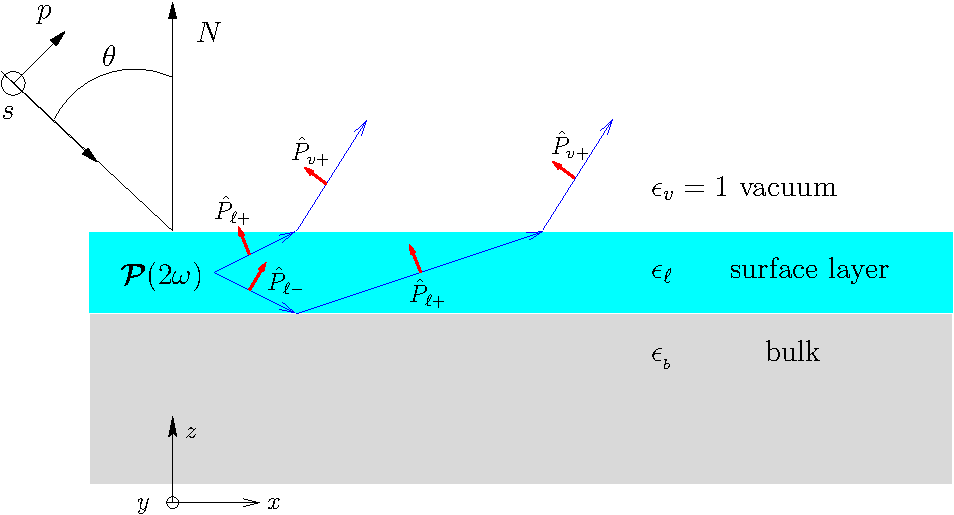
\includegraphics[width=0.5\textwidth]{content/figures/diag-3layer}
\caption{Sketch of the three layer model for SHG. Vacuum is on top with
$\epsilon_v=1$, the layer with nonlinear polarization 
$\boldsymbol{\mathcal{P}}(2\omega)$
is characterized with $\epsilon_{\ell}(\omega)$ and the bulk with
$\epsilon_{b}(\omega)$. In the dipolar approximation the bulk does not radiate
SHG. The thin arrows are along the direction of propagation, and the unit
vectors for $p$-polarization are denoted with thick arrows (capital letters
denote SH components). The unit vector for $s$-polarization points along $-y$
(out of the page).\label{fig:3layer}}
\end{figure}

To describe the propagation of the SH field, we see from Fig. \ref{fig:3layer},
that it is refracted at the layer-vacuum interface ($\ell v$), and  reflected
from the layer-bulk ($\ell b$) and layer-vacuum ($\ell v$) interfaces, thus we
define
\begin{equation}\label{r5}
\mathbf{T}^{\ell v}
= \hat{\mathbf{s}}T_{s}^{\ell v}\hat{\mathbf{s}} 
+ \hat{\mathbf{P}}_{v+}T_{p}^{\ell v}\hat{\mathbf{P}}_{\ell +},
\end{equation}
as the tensor for transmission from the $\ell v$ interface,
\begin{equation}\label{r6}
\mathbf{R}^{\ell b}
= \hat{\mathbf{s}}R_{s}^{\ell b}\hat{\mathbf{s}}
+ \hat{\mathbf{P}}_{\ell +}R_{p}^{\ell b}\hat{\mathbf{P}}_{\ell -},
\end{equation} 
as the tensor of reflection from the $\ell b$ interface, and
\begin{equation}\label{r6b}
\mathbf{R}^{\ell v}
= \hat{\mathbf{s}}R_{s}^{\ell v}\hat{\mathbf{s}}
+ \hat{\mathbf{P}}_{\ell -}R_{p}^{\ell v}\hat{\mathbf{P}}_{\ell +},
\end{equation} 
as that from the $\ell v$ interface. The Fresnel factors in uppercase letters,
$T^{ij}_{s,p}$ and $R^{ij}_{s,p}$, are evaluated at $2\omega$ from the following
well known formulas,\cite{ mizrahiJOSA88}
\begin{align}
t_s^{ij}(\omega) &=
\frac{2w_{i}(\omega)}{w_{i}(\omega)+w_{j}(\omega)},\\
t_{p}^{ij}(\omega) &=
\frac{2w_{i}(\omega)\sqrt{\epsilon_{i}(\omega)\epsilon_j(\omega)}}
     {w_{i}(\omega)\epsilon_{j}(\omega)+w_{j}(\omega)\epsilon_{i}(\omega)},\\
r_s^{ij}(\omega) &=
\frac{w_{i}(\omega) - w_{j}(\omega)}
     {w_{i}(\omega) + w_{j}(\omega)},\\
r_{p}^{ij}(\omega) &=
\frac{w_{i}(\omega)\epsilon_{j}(\omega) - w_{j}\epsilon_{i}(\omega)}
     {w_{i}(\omega)\epsilon_{j}(\omega) + w_{j}(\omega)\epsilon_{i}(\omega)}. 
\end{align}
From these expressions one can show that,
\begin{align}\label{mf}
1 + r^{\ell b}_{s} &= t^{\ell b}_{s}\nonumber\\
1 + r^{\ell b}_{p}
&= \frac{n_b}{n_\ell} 
t^{\ell b}_{p} 
\nonumber\\ 
1 - r^{\ell b}_{p}
&= \frac{n_\ell}{n_b}
   \frac{w_{b}}{w_{\ell}}t^{\ell b}_{p}\\ 
t^{\ell v}_{s,p} &= \frac{w_{\ell}}{w_{v}}t^{v\ell}_{s,p}\nonumber
.
\end{align}

%%%%%%%%%%%%%%%%%%%%%%%%%%%%%%%%%%%%%%%%%%%%%%%%%%%%%%%%%%%%%%%%%%%%%%%%%%%%%%%%
%%%%%%%%%%%%%%%%%%%%%%%%%%%%%%%%%%%%%%%%%%%%%%%%%%%%%%%%%%%%%%%%%%%%%%%%%%%%%%%%


\subsection{SSHG Yield}\label{sec:yield}

We obtain the total $2\omega$ radiated field by using Eqs. \eqref{r5},
\eqref{r6}, and \eqref{r6b},
\begin{equation*}\label{r7}
\mathbf{E}(2\omega)
= E_s(2\omega)
\left(
\mathbf{T}^{\ell v} + \mathbf{T}^{\ell v}\cdot\mathbf{R}^{\ell b}
\right)
\cdot\hat{\mathbf{s}}
+ E_{p+}(2\omega)\mathbf{T}^{\ell v}\cdot\hat{\mathbf{P}}_{\ell +}
 + E_{p-}(2\omega)\mathbf{T}^{\ell v}
\cdot\mathbf{R}^{\ell b}\cdot\hat{\mathbf{P}}_{\ell-}.
\end{equation*}
The first term is  the transmitted $s$-polarized field, the second one is the
reflected and then transmitted $s$-polarized field and the third and fourth
terms are the equivalent fields for $p$-polarization. The transmission is from
the layer into vacuum, and the reflection between the layer and the bulk. After
some simple algebra, we obtain
\begin{equation}\label{r8}
\mathbf{E}_{\ell}(2\omega) = \frac{\gamma i\tilde{\Omega}}{W_{\ell}}
\mathbf{H}_{\ell}\cdot\boldsymbol{\mathcal{P}}_\ell(2\omega),
\end{equation}
where,
\begin{equation}\label{r9}
\mathbf{H}_{\ell}
= \hat{\mathbf{s}}\,T_s^{\ell v}\left(1+R_s^{\ell b}\right)\hat{\mathbf{s}}
+ \hat{\mathbf{P}}_{v+}T_{p}^{\ell v}
\left(
\hat{\mathbf{P}}_{\ell +} +R_{p}^{\ell b}\hat{\mathbf{P}}_{\ell -}
\right). 
\end{equation}
The magnitude of the radiated SH field is given by
$E(2\omega)=\hat{\mathbf{e}}^{\mathrm{F}}\cdot\mathbf{E}_\ell(2\omega)$, where
$\hat{\mathbf{e}}^{\mathrm{F}}$ is the unit vector of the final polarization,
with $\mathrm{F}=S,P$, and then, $\hat{\mathbf{e}}^S=\hat{\mathbf{s}}$ and
$\hat{\mathbf{e}}^P=\hat{\mathbf{P}}_{v+}$. We expand the second term in
parenthesis of Eq. \eqref{r9} as
\begin{equation*}\label{m1}
\begin{split}
\hat{\mathbf{P}}_{\ell +} + R_{p}^{\ell b}\hat{\mathbf{P}}_{\ell -}
&= \frac{\sin\theta_{0}\hat{\mathbf{z}} - W_{\ell}\hat{\boldsymbol{\kappa}}}
        {N_{\ell}}
 + R_{p}^{\ell b}
   \frac{\sin\theta_{0}\hat{\mathbf{z}} + W_{\ell}\hat{\boldsymbol{\kappa}}}
        {N_{\ell}}
\\\nonumber
&= \frac{1}{N_{\ell}}
\left(
\sin\theta_{0}(1+R^{\ell b}_{p})\hat{\mathbf{z}}
- W_{\ell}(1-R^{\ell b}_{p})\hat{\boldsymbol{\kappa}} 
\right)
\\\nonumber 
&= \frac{T^{\ell b}_{p}}{N^{2}_{\ell}N_{b}}
\left(
  N^{2}_{b}\sin\theta_{0}\hat{\mathbf{z}} 
- N^{2}_{\ell}W_{b}\hat{\boldsymbol{\kappa}}
\right)
,
\end{split}
\end{equation*}
and rewrite Eq. \eqref{r8} as
\begin{equation}\label{r10}
E(2\omega) =
\frac{2\gamma i \omega}{cW_{\ell}}
\hat{\mathbf{e}}^{\mathrm{F}}
\cdot
\mathbf{H}_{\ell}
\cdot
\boldsymbol{\mathcal{P}}_\ell(2\omega) 
= \frac{2\gamma i \omega}{cW_{v}}
\mathbf{e}^{\,2\omega,\mathrm{F}}_{\ell}
\cdot\boldsymbol{\mathcal{P}}_\ell(2\omega),
\end{equation}
where
\begin{equation}\label{r12mm}
\mathbf{e}^{2\omega,\mathrm{F}}_{\ell} =
\hat{\mathbf{e}}^{\mathrm{F}}\cdot 
\Bigg[
\hat{\mathbf{s}}T_{s}^{v\ell}T_{s}^{\ell b}\hat{\mathbf{s}} + 
\hat{\mathbf{P}}_{v+}
\frac{T^{v\ell}_{p}T^{\ell b}_{p}}
     {N^{2}_{\ell}N_{b}}
\left(
  N^{2}_{b}\sin\theta_{0}\hat{\mathbf{z}}
- N^{2}_{\ell}W_{b}\hat{\boldsymbol{\kappa}}
\right)
\Bigg].
\end{equation}

In the three layer model the nonlinear polarization is located in layer
$\ell$, thus, we evaluate the fundamental field required in Eq. \eqref{tres}
in this layer as well. We write
\begin{equation}\label{m2}
\begin{split}
\mathbf{E}_{\ell}(\omega)=E_0\left(
\hat{\mathbf{s}} t^{v\ell}_s(1+r^{\ell b}_s)\hat{\mathbf{s}}
+
\hat{\mathbf{p}}_{\ell-}
 t^{v\ell}_{p}
\hat{\mathbf{p}}_{v-}
+
\hat{\mathbf{p}}_{\ell+}
t^{v\ell}_{p}r^{\ell b}_{p}
\hat{\mathbf{p}}_{v-}
\right)\cdot\hat{\mathbf{e}}^{\mathrm{in}}=E_0\mathbf{e}^\omega_{\ell}
,
\end{split}
\end{equation} 
and following the steps that lead to Eq. \eqref{r12mm}, we find that
\begin{equation}\label{m12}
\mathbf{e}^{\omega,\mathrm{i}}_{\ell}
= \left[
\hat{\mathbf{s}}t_{s}^{v\ell}t_{s}^{\ell b}\hat{\mathbf{s}} 
+ \frac{t^{v\ell}_{p}t^{\ell b}_{p}}
       {n^{2}_{\ell}n_{b}}
\left(
  n^{2}_{b}\sin\theta_{0}\hat{\mathbf{z}}
+ n^{2}_{\ell}w_{b}\hat{\boldsymbol{\kappa}}
\right)
\hat{\mathbf{p}}_{v-}
\right]
\cdot\hat{\mathbf{e}}^{\mathrm{i}}.
\end{equation}

We pause here to reduce this result to the case where the nonlinear polarization
$\mathbf{P}(2\omega)$ radiates from vacuum instead from the layer $\ell$. For
such case we simply take $\epsilon_{\ell}(2\omega) = 1$ and $\ell = v$ ($T^{\ell
v}_{s,p} = 1$), to get
\begin{equation}\label{eq:r13}
\mathbf{e}^{\,2\omega}_{v} = \hat{\mathbf{e}}^{\mathrm{F}}\cdot
\left[
\hat{\mathbf{s}}T_{s}^{v b}\hat{\mathbf{s}} + \hat{\mathbf{P}}_{v+}
\frac{T^{v b}_{p}}{\sqrt{\epsilon_{b}(2\omega)}}
\left(
  \epsilon_{b}(2\omega)\sin\theta_{0}\hat{\mathbf{z}}
- W_{b}\hat{\boldsymbol{\kappa}}
\right) 
\right],
\end{equation}
which agrees with Eq. (3.10) of Ref. \cite{mizrahiJOSA88}.

In the 3-layer model the SH polarization $\boldsymbol{\mathcal{P}}(2\omega)$ is
located in layer $\ell$, where we evaluate the fundamental field required in Eq.
\eqref{eq:tres}. We write
\begin{equation}\label{eq:m2}
\begin{split}
\mathbf{E}_{\ell}(\omega) 
&= E_{0}
\left(
  \hat{\mathbf{s}} t^{v\ell}_{s}(1+r^{\ell b}_{s})\hat{\mathbf{s}}
+ \hat{\mathbf{p}}_{\ell-}t^{v\ell}_{p}\hat{\mathbf{p}}_{v-}
+ \hat{\mathbf{p}}_{\ell+}t^{v\ell}_{p}r^{\ell b}_{p}\hat{\mathbf{p}}_{v-}
\right)
\cdot\hat{\mathbf{e}}^{\mathrm{i}}\\
&= E_{0}\mathbf{e}^\omega_{\ell},
\end{split}
\end{equation} 
where $\hat{\mathbf{e}}^{\mathrm{i}}$ is the $s$ ($\hat{\mathbf{s}}$) or $p$
($\hat{\mathbf{p}}_{v-}$) incoming polarization of the fundamental electric
field. This field is composed of the transmitted field and its first reflection
from the $\ell b$ interface for $s$ and $p$ polarizations. The fundamental
field, once inside the layer $\ell$ will be reflected multiple times at the
$\ell v$ and $\ell b$ interfaces. However, each reflection will diminish the
intensity of the fundamental field. As the SSHG yield scales with the square of
this field, the contribution of the subsequent reflections after the one
considered in Eq. \eqref{eq:m2} can be safely neglected. From Eq. \eqref{eq:mf}
we find that
\begin{equation}\label{eq:m12}
\mathbf{e}^{\omega}_{\ell} =
\left[
  \hat{\mathbf{s}}t_{s}^{v\ell}t_{s}^{\ell b}\hat{\mathbf{s}} 
+ \frac{t^{v\ell}_{p}t^{\ell b}_{p}}{n^{2}_{\ell} n_{b}}
\left(
  n^{2}_{b}\sin\theta_{0}\hat{\mathbf{z}} 
+ n^{2}_{\ell} w_b\hat{\boldsymbol{\kappa}}
\right)
\hat{\mathbf{p}}_{v-}
\right]
\cdot\hat{\mathbf{e}}^{\mathrm{in}}.  
\end{equation}  
To connect with the work in Ref. \cite{mizrahiJOSA88}, we evaluate the fields in
the bulk instead of the layer $\ell$and simply take $n_{\ell} = n_{b}$
$(t^{\ell b}_{s,p} = 1)$, to obtain
\begin{equation}\label{eq:m13}
\mathbf{e}^{\omega}_{b} =
\left[
  \hat{\mathbf{s}}t_{s}^{vb}\hat{\mathbf{s}}
+ \frac{t^{vb}_{p}}{n_{b}}
\left(\sin\theta_{0}\hat{\mathbf{z}} + w_b\hat{\boldsymbol{\kappa}}\right) 
\hat{\mathbf{p}}_{v-}
\right]
\cdot\hat{\mathbf{e}}^{\mathrm{in}},  
\end{equation} 
that is in agreement with Eq. (3.5) of Ref. \cite{mizrahiJOSA88}.

Replacing $\mathbf{E}(\omega)\to E_0\mathbf{e}^{\omega,\mathrm{i}}_\ell$,  
in Eq. \eqref{tres}, we obtain that
\begin{equation}\label{m4}
\boldsymbol{\mathcal{P}}_\ell(2\omega) = 
\left\{
\begin{array}{cc}  
E^{2}_{0}\,\boldsymbol{\chi}:
\mathbf{e}^{\omega,\mathrm{i}}_{\ell}\mathbf{e}^{\omega,\mathrm{i}}_{\ell}
& \text{(cgs units)} \\\\
\epsilon_{0}E^{2}_{0}\,\boldsymbol{\chi}:
\mathbf{e}^{\omega,\mathrm{i}}_{\ell}\mathbf{e}^{\omega,\mathrm{i}}_{\ell}
& \text{(MKS units)} \\
\end{array}
\right.,
\end{equation}
where $\mathbf{e}^{\omega,\mathrm{i}}_{\ell}$ is given by Eq. \eqref{m12},
and thus
Eq. \eqref{r10} reduces to ($W_{v}=\cos\theta_{0}$)
\begin{equation}\label{mr10}
E(2\omega) =
\frac{2\eta i \omega}{c\cos\theta_{0}}
\mathbf{e}^{2\omega,\mathrm{F}}_{\ell}\cdot\boldsymbol{\chi}:
\mathbf{e}^{\omega,\mathrm{i}}_{\ell}\mathbf{e}^{\omega,\mathrm{i}}_{\ell}
,
\end{equation}
where $\eta=2\pi$ for cgs units and $\eta=1/2$ for MKS units. For ease of
notation, we define
\begin{equation}\label{mc0}
\Upsilon_{\mathrm{iF}}
\equiv 
\mathbf{e}^{2\omega,\mathrm{F}}_{\ell}\cdot\boldsymbol{\chi}:
\mathbf{e}^{\omega,\mathrm{i}}_{\ell}\mathbf{e}^{\omega,\mathrm{i}}_{\ell}
.
\end{equation}
From Eqs. \eqref{uno},
\eqref{dos}, and \eqref{mr10} we obtain that
\begin{equation}\label{mc6}
\mathcal{R}_{\mathrm{iF}}
=\frac{\eta\omega^{2}}{c^{3}\cos^{2}\theta_{0}}
\left\vert  
\frac{1}{n_{\ell}}
\Upsilon_{\mathrm{iF}}
\right\vert^{2},
\end{equation}
as the SSHG yield, where $\eta =32\pi^3$ for cgs units and
$\eta=1/(2\epsilon_0)$ in MKS units. Since $\boldsymbol{\chi}$ is a surface
second order nonlinear susceptibility, in the MKS unit system is given in
$\mathrm{m}^{2}/\mathrm{V}$, and thus $\mathcal{R}_{\mathrm{iF}}$ is given in
$\mathrm{m}^{2}/\mathrm{W}$.

It is worth mentioning that we can easily recover the results from Ref.
\cite{mizrahiJOSA88}, which are in turn equivalent to those in Ref.
\cite{sipePRB87}. We simply take
$\mathbf{e}^{2\omega}_{\ell}\to\mathbf{e}^{2\omega}_{v}$,
$\mathbf{e}^{\omega}_{\ell}\to\mathbf{e}^{\omega}_{b}$, and we have
\begin{equation}\label{eq:m69}
\mathcal{R}_{\mathrm{iF}}(2\omega) =
\frac{\eta\omega^{2}}{c^{3}\cos^{2}\theta_{0}}
\left\vert\mathbf{e}^{\,2\omega}_{v}\cdot
\boldsymbol{\chi}:\mathbf{e}^{\omega}_{b}\mathbf{e}^{\omega}_{b}
\right\vert^{2}.
\end{equation}
This is the SSHG yield  of a nonlinear polarization sheet radiating from the
vacuum region above the surface, with the fundamental field evaluated below the
surface in the bulk of the material characterized by $\epsilon_{b}(\omega)$.

\stopcontents[chapters]
